\chapter[Analysis]{Overview of the Charge Asymmetry Analysis}

This chapter will describe in detail the methedology used in the measurements
presented in the following chapters. 

\section{Event Selection}

The event selection is performed single electron datasets. 

These datasets are formed of events that are selected using various single photon and single
electron triggers. From these datasets, electrons are selected that pass a limited
number of cuts. Events that contain only a single electron are then selected for
the analysis.

\subsection{Trigger}

\todo{I don't like this}

In the following analysis, a control region is obtained by inverting the $\Delta\phi$ and
$\Delta\eta$ variables. To ensure that this inverted selection will select
events, it is necesary to avoid using triggers that apply a selection on these
variables whenever possible.

\subsection{Electron Selection}

Electrons candidates are identified using a cut based approach on an limited
number of variables. The cut values used correspond to the \unit{80}{\%}
working point from \TableRef{tab:electronwp}, and are summarised again in
\TableRef{tab:elecuts}. The \unit{80}{\%} working point was chosen as a
compromise between ensuring suitable statistics while maintaining the purity of
the sample.

\begin{table}[htbp]
  \begin{center}
    \leavevmode
    \begin{tabular}{lll} 
    \toprule
      Selection Variable & \multicolumn{2}{c}{Cut Value}\\
                         & Barrel & Endcap\\
      \midrule
      \multicolumn{3}{l}{\emph{ID Cuts}}\\ 
        H/E & 0.04 & 0.025 \\
        $\Delta\phi$ & 0.06 & 0.03 \\
        $\Delta\eta$ & 0.004 & 0.007  \\
        $\sigma_{\eta\eta}$ & 0.01 & 0.03 \\ \midrule
      \multicolumn{3}{l}{\emph{Isolation Cuts}}\\
        $ISO_{trk} / E_T $  & 0.09 & 0.04 \\
        $ISO_{ecal}/ E_T$  & 0.07 & 0.05 \\
        $ISO_{hcal}/ E_T$  & 0.10 & 0.025 \\ \midrule
      \multicolumn{3}{l}{\emph{Conversion Rejection Cuts}}\\ 
        Missing Hits  & \multicolumn{2}{c}{$\leq 0$}\\
        Dist $||$ Dcot   & \multicolumn{2}{c}{$>0.02$}\\
    \bottomrule
    \end{tabular}
    \caption{\label{tab:elecuts} Electron selection variables and corresponding cut values.}
  \end{center}
\end{table}

Incorrectly assigning the charge of an electron will lead to a diltuion of the
measured charge asymmetry, to overcome this an additional requirement is applied
to the charge of the reconstructed electron. The methods for assigning a charge
to an electron are described in \SectionRef{sec:charge}. The methods are based
on the GSF electron charge, the general track charge and the supercluster
charge.

The incorrect charge assignment rate can be measured at the Z peak by comparing the same
sign \HepProcess{\PZ\to\Pepm\Pepm} yield to the oposite sign
\HepProcess{\PZ\to\Pepm\Pemp} yield. \FigureRef{fig:zpeak} show these Z yields
using only the \ac{GSF} track charge (black) and also requiring a unaminous
asignment of charge from all three methods (red). 

The incorrect charge assignment rate from the GSF track charge alone is about
\unit{3}{\%}.  By requiring that all three methods for assigning the charge
agree, and vetoing events otherwise, the incorrect assignment rate can be
reduced by a factor of 8 with only a \unit{5}{\%} loss in efficiency.

\begin{figure}[htbp]
  \centering
  \begin{subfigure}{\textwidth}
    \centering
    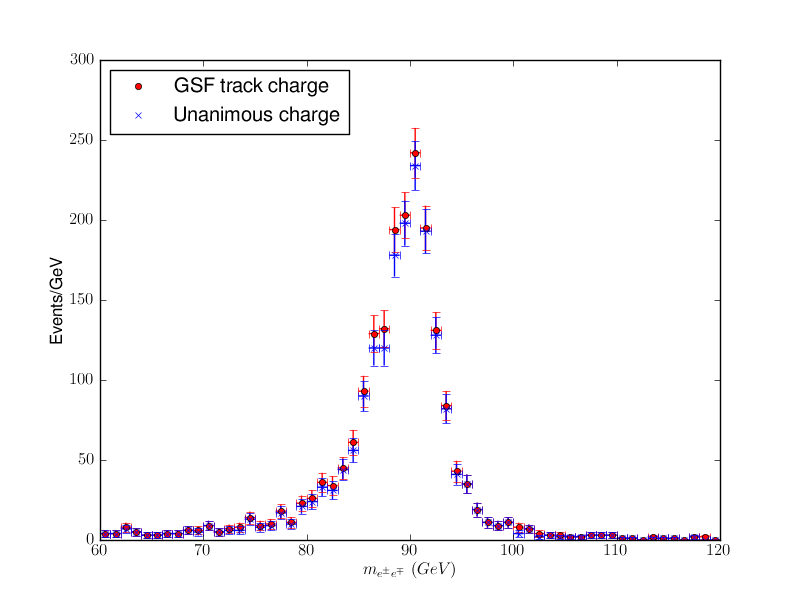
\includegraphics[width=0.85\textwidth]{zpeak_os}
    \caption{Oposite sign \PZ.}
    \label{fig:zpeak_os}
  \end{subfigure}
  \begin{subfigure}{\textwidth}
    \centering
    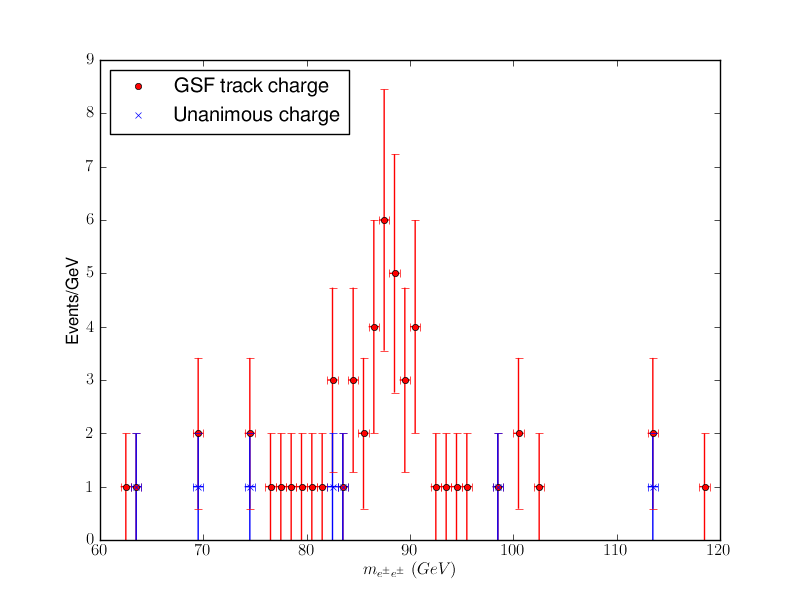
\includegraphics[width=0.85\textwidth]{zpeak_ss}
    \caption{Same sign \PZ.}
    \label{fig:zpeak_ss}
  \end{subfigure}
  \caption{ $Z\rightarrow ee$ peak. One electron is required to be in the
barrel to pass the VBTF80 selection and to have a fraction of energy loss by
radiation less than 0.3; the second electron is required only to pass the VBTF80
selection.}\label{fig:zpeak} 
\end{figure}

\subsection{Event Selection}
An Event is selected if it contains a single electron that passes all the electron
selection requirements.
To remove Drell-Yan events, an event is vetoed if it contains a second lepton
(an electron passing a loose selecton, or an isolated muon) with $\PT > 
\unit{15}{\GeV}$.

\section{Signal Yield Extraction}
The number of signal and background events in each bin is extracted using a fit
to the \ETm distribution using two templates.
The first is the sum of the \Wenu signal and the \ac{EWK} background shapes,
and the second is the sum of the \ac{QCD} plus \gjet processes.

\subsection{\ac{QCD} \ETm Shape}
The \ac{QCD} and \gjet background distribution is obtained from a control sample of
events. The control sample is selected by requiring that the electrons pass the
isolation and H over E cuts but fail the $\Delta\phi$ and $\Delta\eta$ cuts as
shown in \TableRef{asym36:antisel}.

\begin{figure}[htbp]
  \centering
  \begin{subfigure}{0.45\textwidth}
    \centering
    \includegraphics*[trim = 0mm 0mm 15mm 0mm, clip, width=\textwidth, angle=90]{MetCompare_anti_eta1.pdf}
    \caption{test.}
    \label{fig:qcd_met_eta1}
  \end{subfigure}
  \begin{subfigure}{0.45\textwidth}
    \centering
    \includegraphics*[trim = 0mm 0mm 15mm 0mm, clip, width=\textwidth, angle=90]{MetCompare_anti_eta2.pdf}
    \caption{test.}
    \label{fig:qcd_met_eta2}
  \end{subfigure}
  \begin{subfigure}{0.45\textwidth}
    \centering
    \includegraphics*[trim = 0mm 0mm 15mm 0mm, clip, width=\textwidth, angle=90]{MetCompare_anti_eta3.pdf}
    \caption{test.}
    \label{fig:qcd_met_eta3}
  \end{subfigure}
  \begin{subfigure}{0.45\textwidth}
    \centering
    \includegraphics*[trim = 0mm 0mm 15mm 0mm, clip, width=\textwidth, angle=90]{MetCompare_anti_eta4.pdf}
    \caption{test.}
    \label{fig:qcd_met_eta4}
  \end{subfigure}
  \begin{subfigure}{0.45\textwidth}
    \centering
    \includegraphics*[trim = 0mm 0mm 15mm 0mm, clip, width=\textwidth, angle=90]{MetCompare_anti_eta5.pdf}
    \caption{test.}
    \label{fig:qcd_met_eta5}
  \end{subfigure}
  \begin{subfigure}{0.45\textwidth}
    \centering
    \includegraphics*[trim = 0mm 0mm 15mm 0mm, clip, width=\textwidth, angle=90]{MetCompare_anti_eta6.pdf}
    \caption{test.}
    \label{fig:qcd_met_eta6}
  \end{subfigure}
  \caption{The \ETm distribution on antiselected \ac{MC} simulated events and selected \ac{QCD} and \gjet events in each pseudorapidity bin.}
  \label{asym36:antiselclosure}
\end{figure}

\begin{table}[htbp]
  \begin{center}
    \leavevmode
    \begin{tabular}{lcc} 
    \toprule
      \multicolumn{1}{c}{Variable} & \multicolumn{1}{c}{cut value (barrel)}& \multicolumn{1}{c}{cut value (endcap)}\\\midrule
        H/E & 0.04 & 0.025 \\
        $\Delta\phi$ & $>0.06$  & $>0.04$ \\
        $\Delta\eta$ & $>0.007$ & $>0.009$\\
        $ISO_{trk} / E_T $ & 0.09 & 0.04 \\
        $ISO_{ecal}/ E_T$  & 0.07 & 0.05 \\
        $ISO_{hcal}/ E_T$  & 0.10 & 0.025\\ 
    \bottomrule
    \end{tabular}
    \caption{\label{tab:AScuts}Electron anti-selection variables and corresponding cut values. $\Delta\phi$ and $\Delta\eta$ cuts are inverted.}
  \end{center}
\end{table}

To validate the antiselection used, \ac{QCD} \ac{MC} samples are used. The
distribution of \ac{QCD} events passing the event selection are comapred to the
antselected MC events. This is shown for each eta bin in
\FigureRef{asym36:antiselclosure}.

\subsection{Signal \ETm Shape from Boson Recoil}
The signal \ETm shape is obtained by modeling the recoil of the W boson. 
The recoil response and resolution in \HepProcess{\PZ\to\Plepton\Plepton} data
events is measured as a function of the \pT of the boson. This is combined with
information from the \PW and \PZ \ac{MC} simulation to derive a correction to
the simulation \ETm as a function of \PW \pT.

The modeling of the \HepProcess{\PW\to\Plepton\Pnu} \ETm with boson recoil is
described in detail here \cite{NULL}, and the ntuples containing
\HepProcess{\PW\to\Pelectron\Pnu} simulation with the recoil corrected \ETm were
provided from here \cite{NULL}.

\todo{ALOT MORE}

\subsection{\ac{EWK} \ETm Shape}
The EWK background processes that can produce a single isolated
electron which are considered in this analysis are:
\begin{itemize}
\item \HepProcess{\PZ\to\Pelectron\APelectron},
\item \HepProcess{\PZ\to\Ptauon\APtauon},
\item \HepProcess{\PW\to\Ptau\Pnu},
\item \HepProcess{\Ptop\APtop}.
\end{itemize}

The \ac{EWK} background \ETm distributions were obtained from Pythia \ac{MC}
simulations for each pseudorapidity/charge bin.  The scale of the \ac{EWK} shape
is fixed to the signal \ETm shape by the ratio obtained from \ac{MC} samples.

\subsection{Validation of Signal Extraction Method on Simulation}

The signal yield extraction procedure was validated using pseudodata
experiments. 1000 pseudodata experiments were generated with the number of
events expected in \unit{36.1}{\invpb} of data. The signal yields are extracted
in each experiment and the asymmetry is calculated. The distribution of
asymmetries is then fitted with a gaussian.

The width of the gaussian is the statistical uncertainty on the measurement.
The statistical uncertainty can also be estimated from the following formula
\begin{equation}
  \label{asym36:statuncert}
   \frac{d\mathcal{A}_{stat}}{d\eta} =
   \frac{2 \times \sqrt{ 
       \left( \frac{dN^+}{d\eta} \sigma_{\frac{dN^-} {d\eta}}\right)^2 + 
       \left( \frac{dN^-}{d\eta} \sigma_{\frac{dN^+} {d\eta}}\right)^2  }}
   {\left(  \frac{dN^+}{d\eta} +  \frac{dN^-}{d\eta} \right)^{2} } .
\end{equation}

The uncertainty from \EquationRef{asym36:statuncert} evaulated with \ac{MC} truth
values, and the uncertainty measured from pseudodata experiments for an
integrated luminosity of \unit{36.1}{\invpb} are summarised in
\TableRef{asym36:statuncertsum}.

\begin{table}[htbp]
  \begin{center}
    \begin{tabular}{lcc}
    \toprule
    $|\eta|$ range & $\sigma_{A}$ from \EquationRef{asym36:statuncert}. & $\sigma_{A}$ from pseudo-data exp.\\ \midrule
    $0.0<|\eta|<0.4$ & 0.0064 & 0.0062\\
    $0.4<|\eta|<0.8$ & 0.0064 & 0.0064\\
    $0.8<|\eta|<1.2$ & 0.0065 & 0.0065\\
    $1.2<|\eta|<1.4$ & 0.0096 & 0.0104\\
    $1.6<|\eta|<2.0$ & 0.0076 & 0.0079\\
    $2.0<|\eta|<2.4$ & 0.0077 & 0.0077\\
    \bottomrule
    \end{tabular}
  \caption{Expected statistical error as a function of pseudorapidity, for an
  integrated luminosity of \unit{36}{\invpb}. }
  \label{asym36:statuncertsum}
  \end{center}
\end{table}


%For each of the pseudo-data experiments we calulated the pull on the asymmetry measurement.
%The pull is defined as the diffence between the measured asymmetry for a pseudo-data experiment
%and the MC true value divided by the statistical uncertainty, and represents the number of standard deviations away from the true value.
%The distribution of the pulls from 1000 pseudo-data experiments are shown in figure \ref{fig:toyasym_pull}, and are fitted with a gaussian.
%It is expected that the mean of this gaussian is zero for an unbiased measurement and the
%sigma is one for a measurement with well understood statistical uncertainties.

\begin{figure}[htbp]
  \begin{center}
    \includegraphics*[angle=90,width=0.95\textwidth]{toyasym.pdf}
    \caption{\label{fig:toyasym}Measured Asymmetry for 1000 pseudo-data experiments. The distribution of the measured Asymmetry is fitted with a gaussian.}
  \end{center}
\end{figure}

\begin{figure}[htbp]
  \begin{center}
\includegraphics*[angle=90,width=0.95\textwidth]{pullasyTot.pdf}
    \caption{\label{fig:toyasym_pull}Pull on the Asymmetry in 1000 pseudo-data experiments. The distribution of the pull is fitted with a gaussian.}
  \end{center}
\end{figure}

\section{Corrections}

The following section wil describe sources of bias in the measurement that need
to be taken in to account and, if significant, corrected for.

\subsection{Relative Efficiency}

If the reconstruction efficiency of electrons is different to that of positrons
then the measured asymmetry wil be diluted and will need to be corrected for
the relative efficiency.

\begin{equation}
A_{exp}(\eta) = \frac{
                    \frac{dN}{d\eta}(e^+)-
                    \frac{\epsilon^+}{\epsilon^-}\frac{dN}{d\eta}(e^-)
                }
                {
                    \frac{dN}{d\eta}(e^+)+
                    \frac{\epsilon^+}{\epsilon^-}\frac{dN}{d\eta}(e^-)
                }
\end{equation}

The efficiency for electrons and positrons is measured using the tag and probe
method \todo{reference the CMS tag and probe method paper/note}
with a sample of \Zee events from the same datasets used in the analysis. 
The \Zee events offer a high purity source of unbiased electrons with which to
measure the efficiencies.

From the sample of \Zee events a ``tag'' electron is selected with a strict
selection criteria. 
A ``probe'' electron is selected with the same electron selection decribed
earlier.
The invariant mass of the tag-probe pair is required to be
$\unit{60}{\GeV} < M_ee < \unit{120}{\GeV}$ to ensure a high purity sample.

Efficiencies can then be calculated by measuring the signal yield in events
with one tag electron and one probe passing the selection (tag \& pass) and
events where the probe electron fails the selection (tag \& fail).
The signal yield is extracted using an simultaneous maximum likelihood fit to
both the tag \& pass and the tag \& fail samples.

For this analysis the efficiencies are measured in two parts:

\begin{itemize}
    \item GSF tracking efficiency
    \item Identification efficiency, including conversion rejection, unaminous
charge assignment and HLT request.
\end{itemize}

The main systematic errors on the efficiency measurements are the energy scale
and the signal shape used to extract the signal yield. Fortunately, these
errors will cancel in the calculation of the ratio $R_\epsilon$, the difference
on  $R_\epsilon$ introduced by the energy scale and signal shape is negligable
when compared to the statistical uncertainty of the measurement, so only the
statistical uncertainty is propogated to the error in the ratio,
$dR_\epsilon$.

\begin{equation}
  \label{eq:releff}
  \sigma_{\mathcal{A}} =\mathcal{}(R_\epsilon=1) - \mathcal{A}(R_\epsilon=1\pm dR_\epsilon)  \simeq \frac{dR_\epsilon}{2}(1-\mathcal{A}^2)\simeq \frac{dR_\epsilon}{2}
\end{equation}

\subsection{Charge Misassignment}

The charge misassignment rate, $\omega$, is the rate at which electrons are
misasigned as positive charge and identified as positrons, and vice versa. The
misassignment induces a dilution factor to the asymmetry as a function of the
electron pseudorapidity. If it is assumed that the misassignment rate of
electrons to positrons is the same as the rate of positrons to electrons, \ie 

\begin{equation}
  \omega( \HepProcess{\APelectron \to \Pelectron} ) =
  \omega( \HepProcess{\Pelectron \to \APelectron} )
\end{equation}

then the dilution factor is given by $(1-2\omega_\eta)$ and the measured
asymmetry must be corrected by the following relation

\begin{equation}
  A_{exp}(\eta) = (1-2\omega_\eta)
                \frac{
                    \frac{dN}{d\eta}(e^+)-
                    \frac{\epsilon^+}{\epsilon^-}\frac{dN}{d\eta}(e^-)
                }
                {
                    \frac{dN}{d\eta}(e^+)+
                    \frac{\epsilon^+}{\epsilon^-}\frac{dN}{d\eta}(e^-)
                }
\end{equation}

The rate of charge misassignment is obtained from \Zee samples selected with
the same selection used in the analysis. The rate is measured by comparing the
same sign \PZ\ yield (\HepProcess{\PZ\to\Pepm\Pepm}) to the opposite sign \PZ\
yield (\HepProcess{\PZ\to\Pepm\Pemp}).

\section{Other Systematic Effects}
This section will describe the other systematic effects that need to be
accounted for in the measurement.

\subsection{Signal Extraction Method}

The systematic uncertainty due to the siganl extraction method is evaluated be
considering the error introduced be each \ETm tempalte shape used in the fit
separately.

\subsubsection{Background \ETm Shape}

The \ac{QCD} and \gjet \ETm template shape is obtained from a control sample of
events by antiselecting electrons. This may introduce a systematic bias to the
measurement if there is a difference between the anti-selected \ac{QCD} and \gjet
\ETm samples and the selected \ac{QCD} and \gjet samples.

The systematic uncertainty due to the \ac{QCD} and \gjet \ETm shape is evaluated by
varying the anti-selection used to obtain the control sample and observing the
effect that this has on the measured asymmetry.

For each variation on the antiselection, 500 pseudo-data experiments are
generated with the number of events that are expected in \unit{36.1}{\invpb} of
data. The distribution of the measured asymmetry is then fitted with a
gaussian.
The effect that changing the anti-selection has on the mean of the guassian is
studied, the maximum distance from the asymmetry measured with the nominal
anti-selection is taken as an estimate of the systematic uncertainty.

\subsubsection{Signal \ETm Shape from Boson Recoil}

The signam \ETm shape is constructed using information from the boson recoil.
There are three main sources of uncertainty due to the signal template,

\begin{itemize}
    \item the uncertainty in the recoil corrections,
    \item the effect the energy scale has on the recoil corrections,
    \item the uncertainty on the \ac{PDF} used to generate the events that the
recoil corrections are applied to.
\end{itemize}

To evaluate the effect of the uncertainties of the recoil method, the upper and
lower limits on the corrections are used to generate different tempaltes, and
the effect on the measured asymmetry is evaluated as a measure of the
systematic uncertainty.

The recoil method uses generator level \ac{MC} simulation as an input to the
template shape. To evaluate the efect of the generator used, templates are
generated with the CTEQ 6.6 \todo{cite the CTEQ guys here}
uncertainty \acp{PDF} which contain the central \ac{PDF} and 44 error \acp{PDF}
which contain the \unit{95}{\%} \ac{CL} for each of the 22 free parameters in
the \ac{PDF}. The maximum change in distance with respect to the central value
is taken as a measure of the systematic uncertainty.

Any differences in the energy scale of the electrons between data and \ac{MC}
must be taken in to account to ensure accurate \ETm predictions. The \ac{MC} energy
scale corrections were determined from \PZ data and applied to the \PZ \ac{MC}
before calculating the recoil components \cite{recoil}.

\subsubsection{\ac{EWK} \ETm Shape}

The \ac{EWK} shape is also generated from \ac{MC} samples. During the fitting
procedure, the \ac{EWK} shape is fixed to the \Wenu signal shape according to
the cross section taken from the \ac{MC} samples. To estimate the effect of the
uncertainty of the cross section has on the asymmetry measurement, the \ac{EWK}
background is artificially varied by \unit{$\pm20$}{ \% } and the effect on the
asymmetry is measured. Even with an over estimation of the uncertainty on the
cross section, the effect on the asymmetry is found to be small.

\subsection{Lepton Energy Scale and Resolution}

The energy resolution and scale of the electrons can introduce a systematic
error on the asymmetry due to the effect of of the transverse momentum cut
applied to the electrons. The largest source of electron scale bias is the
radiation induced change to the ECAL crystal transparency.

To correct fot this effect, energy scale and resolution corrrections are
derrived using a \Zee mass distribution. The corrections are parameterised by
six energy scale factors, $s_i$, and six resolutions, $\sigma_i$, one for each
pseudorapidity bin in the asymmetry measurement.
The scale factors represent the average factor each electrons \Pt in data
should be corrected to match the expected \ac{MC} energy scale.
The resolution factors represent the difference of the resolution in data and
\ac{MC}. It is the additional smearing that would need to be applied to
reconstruction level \ac{MC} to match the observed resolution in data.

A sample of \Zee events is  split in to 21 categories which correspond to all
combinations of pseudorapidity bins of the two electrons ($6+\binom{6}{2} = 21$).

A mass template s obtained in each category from \ac{MC} simulation where a
perfect \ac{ECAL} calibration is considered.

A simultaneous fit to the \Zee mass is performed in each of the 21 categories
to determine the six energy scale factors, $s_i$, and the six resolutions, 
$\sigma_i$.

In each category ($category_{ij}$) where one electron is in the $i^{th}$
pseudorapidity bin and the other is in the $j^{th}$ bin, the \ac{MC} template
mass shape is scaled by 

\begin{equation}
    \frac{1}{\sqrt{s_i s_j} } 
\end{equation}

and smeared by an addtional gaussian with width of 

\begin{equation}
    \sqrt{\sigma_i^2+\sigma_j^2}
\end{equation}

%TODO figures
\todo[inline]{Add figures to demonstrate this}

The corrections are applied to the electron before the final \Pt cut so that
the measured asymmetry is corrected for the energy scale.

A conservative uncertainty of \unit{1}{\% } is assigned to the electron energy
after the scale corrections. A systematic error is then estimated by measuring
the difference of the measured charge asymmetry with and without the additional
\unit{1}{\% } scale factor.

